	\documentclass[10pt,oneside]{CBFT_book}
	% Algunos paquetes
	\usepackage{amssymb}
	\usepackage{amsmath}
	\usepackage{graphicx}
	\usepackage{libertine}
% 	\usepackage[bold-style=TeX]{unicode-math}
	\usepackage{lipsum}

	\usepackage{natbib}
	\setcitestyle{square}

	\usepackage{polyglossia}
	\setdefaultlanguage{spanish}


	\usepackage{CBFT.estilo} % Cargo la hoja de estilo

	% Tipografías
	% \setromanfont[Mapping=tex-text]{Linux Libertine O}
	% \setsansfont[Mapping=tex-text]{DejaVu Sans}
	% \setmonofont[Mapping=tex-text]{DejaVu Sans Mono}

	%===================================================================
	%	DOCUMENTO PROPIAMENTE DICHO
	%===================================================================

\begin{document}

\chapter{Ecuaciones de Hamilton-Jacobi}


\section{Introducción a la formulación de Hamilton}

Un sistema mecánico está caracterizado por $\{ q_i, \dot{q}_i \}$ las cuales dan un estado posible del sistema, y además
dan toda la información dinámica del mismo.

Ahora se describirá al sistema en términos de $ q_i, p_i \equiv \partial\Lag/\partial\dot{q}_i$  que tiene la característica
de producir una simetría en la mecánica así definida (la mecánica hamiltoniana).
La simetría es tal que son intercambiables $q_i$ y $p_i$.

Para las ecuaciones de movimiento se parte del hamiltoniano
\[
	\Ham = \sum_i p_i \dot{q}_i - \Lag( q_i, \dot{q}_i, t ),
\]
donde $\Ham =\Ham(q_i,p_i,t)$ tiene la misma información que $\Lag=\Lag(q_i,\dot{q}_i,t)$.

Se puede hacer una analogía con la termodinámica, pues la primer ley se escribe
\[
	dE = dQ - dW = \left. \dpar{E}{S} \right|_V dS - \left. \dpar{E}{V} \right|_S dV,
\]
lo cual implica que usando $S,V$ tengo como ``potencial'' a la energía.
Un estado termodinámico se define por dos variables; $(S,V), (T,P), (S,P), (T,V)$ que son cada par variables conjugadas.

Para definir estos potenciales se usan transformadas de Legendre. Así,
\[
	d(E-TS) = TdS -PdV - TdS -SdT = -PdV - SdT \equiv dA
\]
siendo $A$ la energía libre de Helmholtz.
\[
	d(E+PV) = TdS -PdV + PdV + VdP = TdS + VdP \equiv dH
\]
siendo $H$ la entalpía.

En el caso del Hamiltoniano se tiene 
\[
	d\Ham = \sum_i \dot{q}_i dp_i  + \sum_i p_i d\dot{q}_i - \sum_i \dpar{\Lag}{q_i} dq_i -
	\sum_i d \dpar{\Lag}{\dot{q}_i}\dot{q}_i - \dpar{\Lag}{t}dt 
\]
la cual usando las ecuaciones de Euler-Lagrange y el hecho de que $\partial{\Lag}/\partial{\dot{q}_i} $ es el momento conjugado
$p_i$ se tiene 
\[
	d\Ham = \sum_i \dot{q}_i dp_i  - \sum_i \dot{p}_i dq_i - \dpar{\Lag}{t}dt 
\]
y como esta ecuación es el diferencial total del hamiltoniano se tiene que
\[
	\dpar{\Ham}{t} = -\dpar{\Lag}{t} = \dtot{\Ham}{t}
\]
siendo la última igualdad una derivación vista oportunamente. Asimismo,
\[
	\dpar{\Ham}{p_i} = \sum_i \dot{q}_i \qquad \qquad 
	\dpar{\Ham}{q_i} = -\sum_i \dot{p}_i
\]
que son una mayor cantidad de ecuaciones pero de orden uno (comparando con las ecuaciones del sistema en el formalismo 
lagrangiano).

Con esto definimos un espacio de fases $(p_i,q_i)$ de $2N$ dimensiones para estudiar el movimiento de un sistema de partículas.
En el caso particular de una única partícula tendremos dos variables, $(p,q)$.

\subsection{La idea de Hamilton-Jacobi}

La idea es que se busca una transformación canónica que me transporte a un hamiltoniano nuevo donde toda la solución son 
constantes. Es decir 
\[
	H(q_i,p_i) \longrightarrow K(Q_i,P_i),
\]
donde
\be
	q_i \longrightarrow Q_i \equiv \beta_i \qquad p_i \longrightarrow P_i \equiv \alpha_i
	\label{coord_hamjac}
\ee
% para $\alpha,\beta$ constantes.
Pasamos a unas nuevas coordenadas y momentos $(\beta_i,\alpha_i)$ que son constantes. 
Aunque esto requiere conocer el problema (su solución). Esta transformación existe porque es ir atrás en el tiempo;
la antievolución.

Supongamos una generatriz del tipo $F_2 = S$, llamada {\it función principal de Hamilton}
\[
	S = S(q_i, \alpha_i, t).
\]
Entonces
\be
	\dpar{S}{q_i} = p_i \qquad \dpar{S}{\alpha_i} = \beta_i \qquad \dpar{S}{t} = H - K  
	\label{ecshamjac}
\ee
donde 
\[
	H(q_i,p_i,t) - \dpar{S}{t} = K = 0
\]
que es la condición necesaria para garantizar las condiciones \eqref{coord_hamjac}.
Esto lleva a la ecuación de Hamilton-Jacobi,
\be
	H(q_i,p_i,t) - \dpar{S}{t} = 0
	\label{ecshamjac2}
\ee
que no es otra cosa que una ecuación en derivadas parciales (PDE) al especializar $H$ en las derivadas parciales
\[
	H( q_i, \dpar{S}{q_i}, t) - \dpar{S}{t} = 0,
\]
que son $n+1$ variables y $n+1$ constantes (una es trivial porque la ecuación \eqref{ecshamjac2} no depende de $S$ sino de sus 
derivadas).
Notemos que 
\[
	\dpar{S}{q_i} = p_i(q_i,\alpha_i,t) \qquad \dpar{S}{\alpha_i} = \beta_i(q_i,\alpha_i,t)
\]
y además que Hamilton-Jacobi tiene solución si el problema es totalmente separable.
Si $H=H(q_i,\alpha_i)$ entonces $dH/dt = \partial H/\partial t=0$ y en ese caso es $H=cte.$ y
podemos poner $H=\alpha_1$.
Entonces
\[
	\dpar{S}{t} = -\alpha_1 \quad \longrightarrow \quad S=W(q_i,\dpar{S}{q_i}) -\alpha_1 t .
\]

Se procede en la misma forma con cada coordenada hasta obtener $S$.

Podemos ver que si $\alpha_1 = \alpha_1(\alpha_i)$, y me quedo con $H=\alpha_1 \equiv K$ entonces
\[
	\dpar{K}{\alpha_i} = a = \dot{Q}_i \longrightarrow Q_i = \beta = a t + \beta_0 
\]
\[
	\dpar{K}{\beta_i} = 0 = -\dot{P}_i \longrightarrow P_i = \alpha_i (ctes.).
\]

La $\alpha_1$ no puede depender de $q_i$ pues si se tuviera $\partial \alpha_1 /\partial q_i \neq 0$ 
no sería constante $\alpha_1$ pues $\dot{q}\neq 0$.

Luego, invirtiendo las ecuaciones \eqref{ecshamjac} determinamos las trayectorias
\[
	q_i = q_i(\alpha_i, \beta_i, t).
\]

Además, si el problema es totalmente separable, entonces
\[
	S = \sum_i^N \; W(q_i, \alpha_1,...,\alpha_n) - \alpha_1 t
\]
y tendré tantas constantes de movimiento como grados de libertad. La solución se compone de problemas
independientes en una variable.

% =================================================================================================
\section{Preservación del volumen en una transformación canónica}
% =================================================================================================

Definamos un hipervolumen $\mathcal{V}$ en el espacio de fases de acuerdo a
\[
	\int dq_1 dq_2 ... dq_n dp_1 dp_2 ... dp_n = \mathcal{V}_{p,q}
\]
\[
	\int dQ_1 dQ_2 ... dQ_n dP_1 dP_2 ... dP_n = \mathcal{V}_{P,Q}
\]
\begin{figure}
	\begin{center}
	\includegraphics[width=0.4\textwidth]{images/fig_mc_hamjac2.pdf}	 
	\end{center}
	\caption{}
\end{figure} 
El jacobiano de la transformación es 
\[
	\frac{\partial (Q_1,...,Q_n,P_1,...,P_n)}{\partial (q_1,...,q_n,p_1,...,p_n)} =
	\frac{\partial (Q_1,...,Q_n,P_1,...,P_n)/\partial (q_1,...,q_n,P_1,...,P_n)|_{P_i=cte}}
	{\partial (q_1,...,q_n,p_1,...,p_n)/\partial (q_1,...,q_n,P_1,...,P_n)|_{q_i=cte}}
\]
que en notación de matriz es 
\[
	\begin{pmatrix}
	\dpar{Q_1}{q_1} & \dpar{Q_1}{q_2} & ... & \dpar{Q_1}{p_n} \\
	.. & .. & .. & .. \\
	\dpar{P_n}{q_1} & .. & .. & \dpar{P_n}{p_n}
	\end{pmatrix}
\]
Entonces 
\[
	J_{ij}^{num} = \dpar{Q_i}{q_j} = \frac{\partial}{\partial q_j} \left(\dpar{F_2}{P_i} \right)
\]
y
\[
	J_{ij}^{den} = \dpar{p_i}{P_j} = \frac{\partial}{\partial P_j} \left(\dpar{F_2}{q_i} \right)
\]
pero como estas dos expresiones son iguales se tiene que $J=1$ y entonces se conserva
el volumen, aunque cambiando de forma.

En sistemas de un grado de libertad
\[
	A_{p,q} = \int dp dq \qquad A_{P,Q} = \int dP dQ
\]
y el jacobiano
\[
	J = \begin{vmatrix}
	     \dpar{Q}{q} & \dpar{Q}{p} \\
	     \dpar{P}{q} & \dpar{P}{p}
	    \end{vmatrix} =
	    \dpar{Q}{q} \dpar{P}{p} - \dpar{Q}{p} \dpar{P}{q} = [Q, P] = 1
\]
\begin{figure}
	\begin{center}
	\includegraphics[width=0.6\textwidth]{images/fig_mc_hamjac1gl.pdf}	 
	\end{center}
	\caption{}
\end{figure} 
Notamos que le corchete de Poisson para una transformación canónica en un grado de
libertad es el corchete que ya sabíamos da uno. El área se conserva.

Comentemos que un sistema disipativo achica el área de la transformación.

% =================================================================================================
\section{Variables ángulo-acción}
% =================================================================================================

Consideremos una transformación canónica 
\[
	p,q \longrightarrow J,\theta
\]
la cual requiere
\begin{itemize}
 \item Conservativos $S = W - Et $
 \item Totalmente separables $W = \sum_i^N \; W_i(q_1,\alpha_1,...,\alpha_n)$
 \item Problemas periódicos
\end{itemize}

El movimiento periódico es de rotación o libración,
\begin{figure}[htb]
	\begin{center}
	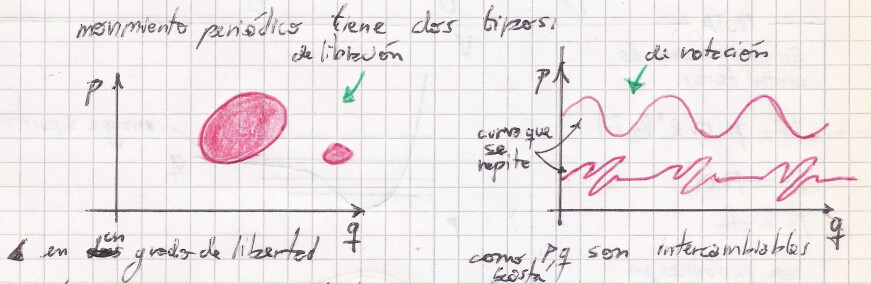
\includegraphics[width=0.7\textwidth]{images/fig_mc_rot_lib.pdf}	 
	\end{center}
	\caption{}
\end{figure} 

La periodicidad de cada coordenada no implica periodicidad de todo el movimiento real.
\[
	S = \sum_i^N \; W_i(q_i,J_i) - Et
\]

Libración y rotación son dos movimientos de naturaleza diferente. No se puede pasar de
uno a otro mediante pequeñas perturbaciones.

\begin{figure}
	\begin{center}
	\includegraphics[width=0.7\textwidth]{images/fig_mc_hamjac.pdf}	 
	\end{center}
	\caption{}
\end{figure} 

La integral de acción es
\[
	J_i = \frac{1}{2\pi}\int_{ciclo} p_i(q_1,\alpha_1,...,\alpha_n) dq_i
\]
donde 
\[
	J_i = J_i(\alpha_1,...,\alpha_n)
\]
son constantes y a su vez los $\alpha_i$ son constantes de separación.
Asimismo $\alpha_i=\alpha_i(J_1,...,J_n)$. 
La transformación $S$ es 
\[
	\dpar{S}{q_i} = p_i = \dpar{W}{q_i} \qquad \dpar{S}{J_i} = \theta_i = \dpar{W}{J_i}
\]
siendo $p_i = p_i(q_1,J_1,...,J_n)$.
El nuevo hamiltoniano es $E=E(J_1,...,J_n)$
\[
	\dpar{E}{J_i} = \dot{\theta}_i \equiv \omega \qquad \dpar{E}{\theta_i} = -\dot{J}_i
\]
de manera que tenemos
\[
	\theta_i = \omega t + \theta_{0_i} \qquad  \dpar{W}{J_i} = \theta_i = \theta_i(q_i, J_i)
\]
y entonces despejamos las $q_i$ desde
\[
	\theta_i(q_i, J_i) = \omega t + \theta_{0_i}.
\]

Las condiciones iniciales $(q_i, J_i)$ se introducen en
\[
	\dpar{W}{q_i} = p_i(q_1,J_1,...,J_n)
\]
y obtengo las $J_1, ..., J_n$ constantes.

% =================================================================================================
\section{Transformación canónica infinitesimal}
% =================================================================================================

Difieren de la identidad en un infinitésimo
\[
	F_2 = 	F_2(q_i,P_i) = \sum_i^N q_iP_i
\]
es la identidad
\[
	\dpar{F_2}{q_i} =  p_i \equiv P_i \qquad \dpar{F_2}{P_i} =  Q_i \equiv q_i
\]
y donde considero
\[
	F_2(q_i,P_i) = \sum q_i P_i + \epsilon G(q_1,...,q_n,P_1,...,P_n) \qquad \textrm{con} \; \epsilon \ll 1
\]
\[
	\dpar{F_2}{q_i} = p_i = P_i + \epsilon\dpar{G}{q_i} \longrightarrow P_i = p_i - \epsilon\dpar{G}{q_i} 
\]
\[
	\dpar{F_2}{P_i} = Q_i = q_i + \epsilon\dpar{G}{P_i} \longrightarrow q_i = Q_i - \epsilon\dpar{G}{P_i} 	
\]
donde $\partial G/\partial P_i \approx \partial G/\partial p_i$ diferirán en un orden $\epsilon^2$ el cual
descarto. Entonces
\[
	\delta p_\ell = -\epsilon \dpar{G}{q_\ell} \qquad \delta q_\ell = \epsilon \dpar{G}{P_\ell}.
\]

Si considero $H$ en lugar de $G$ y $\epsilon = \delta t$ entonces
\[
	\frac{\delta p_\ell}{\delta t} = -\dpar{H}{q_\ell} \qquad \frac{\delta q_\ell}{\delta t} = \dpar{H}{p_\ell}
\]
de tal manera que 
\[
	\dot{p}_\ell = -\dpar{H}{q_\ell} \qquad \dot{q}_\ell = -\dpar{H}{p_\ell}
\]
y donde se ve que el $H$ genera la transformación evolución temporal.
Por otra parte, se puede ver cómo varía una cierta cantidad $A$ ante la transformación canónica.
\[
	\delta A = A(q_i + \delta q_i, p_i + \delta p_i) - A(q_i,p_i)
\]
y
\[
	\delta A = \sum_i \left( \dpar{A}{q_i} \delta q_i + \dpar{A}{p_i} \delta p_i \right)
\]
\[
	\delta A = \epsilon \sum_i \left( \dpar{A}{q_i} \dpar{H}{p_i} - \dpar{A}{p_i} \dpar{H}{q_i} \right) =
	\epsilon[A,H] \longrightarrow \frac{\delta A}{\delta t} = [A,H]
\]
entonces las constantes de movimiento generan transformaciones canónicas infinitesimales que dejan invariante
al hamiltoniano $H$. Si
\[
	\dtot{A}{t} = 0 \Longrightarrow [A,H] = 0
\]

Consideremos una rotación infinitesimal. Una rotación en torno al eje $z$
\[
	\begin{cases}
		x_i' = x_i - \delta \alpha y_i \\
		y_i' = y_i + \delta \alpha x_i \\
		z_i' = z_i
	\end{cases}
\]
que implica 
\[
	\delta x_i = -  \delta \alpha y_i \qquad \qquad \delta y_i = \delta \alpha x_i \qquad \qquad 
	\delta z_i = 0
\]
\notamargen{Las constantes de movimiento están generadas por simetrías (Noether).}

Luego,
\[
	G = \sum_i ( x_i p_{y_i} - y_i p_{x_i} ) = \ell_z
\]
y una rotación en torno a $\hat{n}$ es
\[
	\delta\alpha [ A, \vb{L}\cdot\vb{n} ] = \delta A,
\]
si $A$ es un vector $\vb{V}$ entonces
\[
	\delta\alpha [ \vb{V}, \vb{L}\cdot\vb{n} ] = \delta \vb{V} = \delta\alpha \vb{n} \times \vb{V},
\]
de modo que 
\[
	[ \vb{V}, \vb{L}\cdot\vb{n} ] = \vb{n} \times \vb{V}
\]
es una relación vectorial; es decir que valen
\[
	[ V_x, \vb{L}\cdot\vb{n} ] = (\vb{n} \times \vb{V})_x
\]
y lo mismo para los componentes $y,z$. Además
\[
	[L_x, L_z] = ( \hat{z} \times \vb{L} )_z = - L_y
\]
\[
	[L_y, L_z] = ( \hat{z} \times \vb{L} )_y = L_x
\]
\[
	[L_x, L_y] = ( \hat{y} \times \vb{L} )_x = L_z
\]
o bien 
\[
	[L_i, L_j] = \varepsilon_{ijk} L_k
\]
donde 
\[
	\varepsilon_{ijk} = \begin{cases}
	 0 \quad \text{ si se repite índice } \\
	 1 \quad \text{ si es permutación cíclica } \\
	 -1 \quad \text{ si es permutación anticíclica }
	\end{cases}
\]

Esto nos dice que no podemos elegir como momentos estas constantes de movimiento puesto que el
corchete de Poisson entre ellas es nulo.
No va a existir transformación canónica donde $p_1 = L_x, p_2 = L_y, p_3 = Lz$ pues su corchete de
Poisson entre ellas no se anula.
% =================================================================================================
\section{Potencial electromagnético}
% =================================================================================================

Arranquemos por los momentos canónicamente conjugados
\[
	\dpar{\Lag}{\dot{q}_i} = p_i \quad \textrm{pero} \; si V \neq V(q) \longrightarrow \dpar{T}{\dot{q}_i} = p_i
\]
entonces
\[
	U(q,\dot{q}) =  e \phi - e/c \vb{A}\cdot\vb{V} \longrightarrow \Lag = T - e \phi + e/c  \vb{A}\cdot\vb{V}
\]
\[
	p_x = \dpar{T}{\dot{x}} - \dpar{U}{\dot{x}} = m V_x - (e/c) A_x.
\]

Hacemos un cambio de gauge, en un potencial generalizado
\[
	U =  e \Phi(\vb{x},t) - (q/c) \vb{A}(\vb{x},t)\cdot\vb{V}(t)
\]
y el cambio de gauge es
\[
	\vb{A}' = \vb{A} + \nabla f,
\]
que no altera las ecuaciones de movimiento.


\begin{ejemplo}{\bf Problema de parcial}

El problema cuya geometría se ilustra a continuación. Se consideran $m_1 = m_2 = m$, $m_3 = M$ y  $k$ {\it slinkies}.

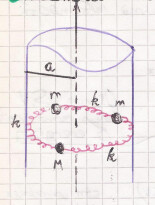
\includegraphics[scale=0.5]{images/fig_mc_problema_parcial_osc_0.jpg}
 
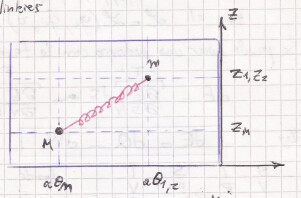
\includegraphics[scale=0.5]{images/fig_mc_problema_parcial_osc_1.jpg}

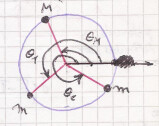
\includegraphics[scale=0.5]{images/fig_mc_problema_parcial_osc_2.jpg}

Es claramente un problema de seis grados de libertad, $\theta_M, \theta_1, \theta_2, Z_M, Z_1, Z_2$ 

Podemos escribir la energía cinética y el potencial como 
\[
	T = \frac{1}{2} M a^2 \dot{\theta}_M^2 + \frac{1}{2} M a^2 (\dot{\theta}_1^2 + \dot{\theta}_2^2 ) +
	\frac{1}{2} M \dot{Z}_M^2 + \frac{1}{2} m ( \dot{Z}_1^2 + \dot{Z}_2^2 )
\]
\[
	V = \frac{1}{2} \left[ a^2 ( \theta_2 - \theta_M ) + ( Z_2 - Z_M )^2 \right] +
	\frac{1}{2} \left[  a^2 ( \theta_1 - \theta_2 ) + ( Z_1 - Z_2 )^2 \right] +
	\frac{1}{2} \left[ a^2 ( \theta_1 - \theta_M ) + ( Z_1- Z_M )^2 \right] 
\]
\[
	\Lag = T - V
\]
Como ya está en forma cuadrática no es necesario aproximar. Si tenemos expresiones lineales habría que desarrollar
a orden dos, por ejemplo $ \cos \theta \sim 1 - \theta^2/2 $ y me quedo con los términos cuadráticos.

Definimos coordenadas referidas al equilibrio. Nos paramos en el equilibrio y oscilamos en torno a él.
\[
 	\eta_1 = ( \theta_M - \theta_{\mbox{eq}} ) 
 	\qquad 
 	\eta_2 = ( \theta_M - \theta_{ 1 \mbox{eq} } )a 
 	\qquad 
 	\eta_3 = ( \theta_2 - \theta_{ 2 \mbox{eq} } )a
\]
\[
	\eta_4 = Z_M - Z_{M\mbox{eq}} \qquad \eta_5 = Z_1 - Z_{1\mbox{eq}} \qquad \eta_6 = Z_2 - Z_{2\mbox{eq}}
\]
con sus correspondientes velocidades
\[
	\dot{\eta}_1 = a \dot{\theta}_M \qquad \dot{\eta}_2 = a \dot{\theta}_1 \qquad \dot{\eta}_3 = a \dot{\theta}_2
\]
\[
	\dot{\eta}_4 = \dot{Z}_M \qquad \dot{\eta}_5 = \dot{Z}_1 \qquad \dot{\eta}_6 = \dot{Z}_2
\]

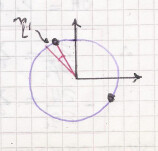
\includegraphics[scale=0.5]{images/fig_mc_problema_parcial_osc_3.jpg}

El lagrangiano será 
\begin{multline*}
	\Lag  =  \frac{1}{2} M \dot{\eta}_1^2 + \frac{1}{2}\dot{\eta}_4^2 + \frac{1}{2} m (\dot{\eta}_2^2 + \dot{\eta}_3^2 + \dot{\eta}_5^2 + \dot{\eta}_6^2 ) \\
	- \frac{k}{2}\left[ (\eta_1 - \eta_2 )^2 + (\eta_5 - \eta_4 )^2 + (\eta_1 - \eta_3 )^2 + (\eta_6 - \eta_4 )^2 + (\eta_2 - \eta_3 )^2 + (\eta_5 - \eta_6 )^2 \right]
\end{multline*}


Habria que identificar los coeficientes para armar $T,V$ en 
\[
	\Lag = \frac{1}{2} \dot{\bar{eta}}^\dagger \mathbb{T} \dot{\bar{eta}} 
	- \frac{1}{2} \bar{eta}^\dagger \mathbb{V} \bar{eta}
\]

Como ejemplo, desarrollemos algún término
\[
	k(\eta_1 - \eta_2)^2 = k \eta_1 \eta_2 - 2k \eta_1 \eta_2 + k \eta_2 \eta_2 =
	k \eta_1 \eta_2 - k \eta_1 \eta_2 -  k \eta_1 \eta_2 + k \eta_2 \eta_2
\]

Las matrices resultan 
\[
	V = \begin{pmatrix}
	     2 k & -k & -k & 0 & 0 & 0 \\
	     -k & 2k & -k & 0 & 0 & 0 \\
	     -k & -k & 2k & 0 & 0 & 0 \\
	     0 & 0 & 0 & 2k & -k & -k \\
	     0 & 0 & 0 & -k & 2k & -k \\
	     0 & 0 & 0 & -k & -k & 2k
	    \end{pmatrix}
\]
\[
	T = \begin{pmatrix}
	     M & 0 & 0 & 0 & 0 & 0 \\
	     0 & m & 0 & 0 & 0 & 0 \\
	     0 & 0 & m & 0 & 0 & 0 \\
	     0 & 0 & 0 & M & 0 & 0 \\
	     0 & 0 & 0 & 0 & m & 0 \\
	     0 & 0 & 0 & 0 & 0 & m 
	    \end{pmatrix}
\]
y como se ve ambas resultan en bloques de Jordan y son cada bloque igual. El a incluido en la coordenada hace que se
obtenga esa forma simétrica.
En
\[
	\mbox{det}( \mathbb{V} - \omega^2 \mathbb{T} )
\]
se reduce a calcular el determinante de la submatriz de 3 $\times$ 3,
\[
	\begin{bmatrix}
	2 k - \omega^2 M & -k & -k \\
	-k & 2 k - \omega^2 m & -k \\
	-k & -k & 2 k - \omega^2 m 
	\end{bmatrix}
\]
que resulta en la ecuación 
\[
	\omega^2 \left( \omega^4 - \omega^2 \left[  \frac{2k}{M} + \frac{2k}{M} \right] +
	\left[ \frac{6k^2}{mM} + \frac{3k^2}{m^2} \right] \right) = 0,
\]
que da 
\[
	\omega_1^2 = 0 \qquad \qquad \omega_2^2 = \frac{2k}{M} + \frac{k}{m} \qquad \qquad \omega_3^2 = \frac{3k}{m} 
\]

Para $\omega^2 = 0$ la ecuación $ (V - \omega^2 T )A^1 = 0 $ se verifica para 
\[
	A^1 = \alpha \begin{pmatrix} 1 \\ 1 \\ 1 \end{pmatrix}
\]
cuya normalización se ajusta con $ {A^\dagger}^1 T A^1 = 1$ o bien 
\[
	\alpha^2 \begin{pmatrix} 1 & 1 & 1 \end{pmatrix}
	\begin{pmatrix}
	 M & 0 & 0 \\
	 0 & m & 0 \\
	 0 & 0 & m
	\end{pmatrix}
	\begin{pmatrix} 1 \\ 1 \\ 1 \end{pmatrix} = 1,
\]
siendo el valor de $\alpha$ dado por 
\[
	\alpha^2 = \frac{1}{2m+M} \qquad \alpha = \frac{1}{ \sqrt{2m+M} }.
\]

Los autovectores son 
\[
	A^1 = \frac{1}{\sqrt{M + 2m}} \begin{pmatrix} 1 \\ 1 \\ 1 \end{pmatrix} \qquad 
	A^2 = \frac{1}{\sqrt{4m^2/M + 2m}} \begin{pmatrix} -2m/M \\ 1 \\ 1 \end{pmatrix} \qquad 
	A^3 = \frac{1}{\sqrt{ 2m }} \begin{pmatrix} 0 \\ 1 \\ -1 \end{pmatrix} \qquad 
\]
 
Los movimientos están dados por

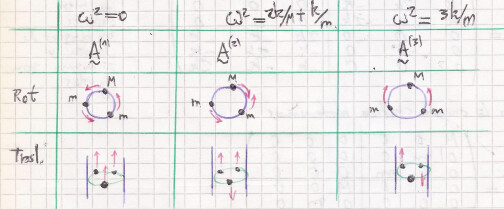
\includegraphics[scale=0.5]{images/fig_mc_problema_parcial_osc_4.jpg}
 
Ahora hay que completar hasta la sexta dimensión
\[
	\bar{\eta}_1 = \frac{1}{\sqrt{2m+M}} \begin{pmatrix} 1 \\ 1 \\ 1 \\ 0 \\ 0 \\ 0
	                                     \end{pmatrix} \qquad \qquad
	\bar{\eta}_3 = \frac{1}{\sqrt{2m}} \begin{pmatrix} 0 \\ 1 \\ -1 \\ 0 \\ 0 \\ 0
	                                     \end{pmatrix} \qquad \qquad
	\bar{\eta}_5 = \frac{1}{\sqrt{2m + 4m^2/M}} \begin{pmatrix} 0 \\ 0 \\ 0 \\ -2m/M0 \\ 1 \\ 1
	                                     \end{pmatrix}
\]
\[
	\bar{\eta}_2 = \frac{1}{\sqrt{2m+ 4m^2/M}} \begin{pmatrix} -2m/M \\ 1 \\ 1 \\ 0 \\ 0 \\ 0 
						\end{pmatrix} \qquad \qquad
	\bar{\eta}_4 = \frac{1}{\sqrt{M + 2m}} \begin{pmatrix} 0 \\ 0 \\ 0 \\ 1 \\ 1 \\ 1
	                                     \end{pmatrix} \qquad \qquad
	\bar{\eta}_6 = \frac{1}{\sqrt{2m}} \begin{pmatrix} 0 \\ 0 \\ 0 \\ 0 \\ 1 \\ -1
	                                     \end{pmatrix}
\] 
 
Luego, para desacoplar la solución habría que plantear la matriz
\[
	\mathbb{B} = [ \eta^\dagger_1 ... \eta_i^\dagger ]
\]
 
\end{ejemplo}

\begin{ejemplo}{\bf Problema 12}

El setup se ilustra en la figura siguiente.

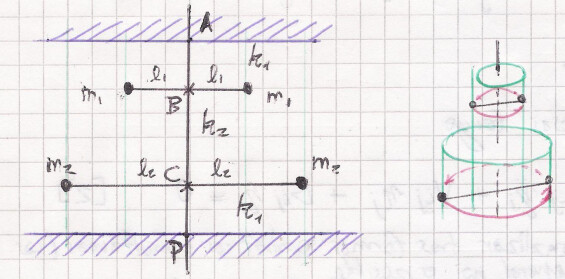
\includegraphics[scale=0.5]{images/fig_mc_problema_12.jpg}

El torque 
\[
	\tau = - k \theta
\]
lo suponemos un potencial $ V = 1/2 k \theta^2 $, donde $k$ tiene unidades de energía.
Las barras solo rotan de manera que 
\[
	T_1 = \frac{1}{2} ( m_1 \ell_1^2 \dot{\theta}_1^2  ) + \frac{1}{2}( m_1 \ell_1^2 \dot{\theta}^2_1 )
\]
donde estamos pensando como dos partículas. En cambio, pensándolo como una barra con momento de inercia es
\[
	T = \frac{1}{2} I \Omega^2
\]

Entonces,
\[
	T = T_1 + T_2 = \frac{1}{2} ( 2 m_1 \ell_1^2 \dot{\theta}_1^2  ) + \frac{1}{2}( 2 m_2 \ell_2^2 \dot{\theta}^2_2 )
\]
\[
	V_1 = \frac{1}{2} k_1 \theta^2_1 \qquad 
	V_{12} = \frac{1}{2} k_2 ( \theta_2 - \theta_1 )^2  \qquad 
	V_2 = \frac{1}{2} k_1 \theta^2_2 
\]

Definiendo $\eta_i = \theta_i - \theta_{\mbox{eq}}$ que implican $\dot{\eta}_i = \dot{\theta}_i $ $(i=1,2)$ se puede escribir el lagrangiano como 
\[
	\Lag = \ell_1^2 m_1 \dot{\eta}_1^2 + \ell_2^2 m_2 \dot{\eta}_2^2 - \frac{1}{2} k_1 \eta_1^2 - \frac{1}{2} k_2 \eta_2^2 - \frac{1}{2} k_2 (\eta_2 - \eta_1)^2
\]
de manera que 
\[
	\mathbb{T} = \begin{pmatrix}
	 2 \ell^2_1 m_1 & 0 \\
	 0 & 2 \ell^2_2 m_2 
	\end{pmatrix}
	\qquad 
	\mathbb{V} = \begin{pmatrix}
	 k_1 + k_2 & - k_2 \\
	 -k_2  & k_1 + k_ 2 
	\end{pmatrix}
\]

Faltaría entonces
\[
	\mbox{det} \{ \mathbb{V} - \omega^2 \mathbb{T} \} = 0
\]
y los autovectores $A^1, A^2$.


\end{ejemplo}

\begin{ejemplo}{\bf Problema 8}

Un problema de pequeñas oscilaciones.

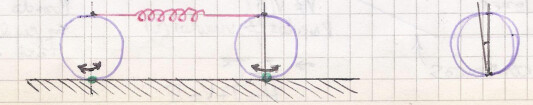
\includegraphics[scale=0.5]{images/fig_mc_problema_8.jpg} 

En este ejemplo hay que suponer que el lagrangiano es ya de entrada de pequeñas oscilaciones.

\end{ejemplo}

\begin{ejemplo}{\bf Problema 1 P96}
 
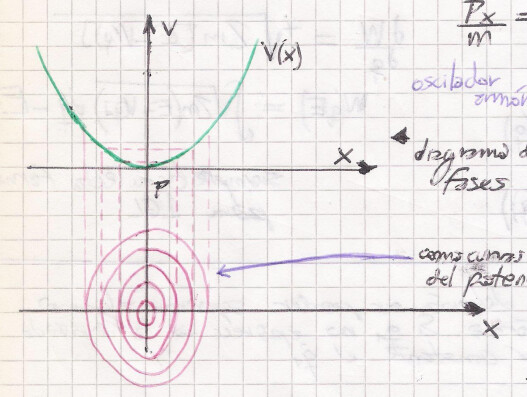
\includegraphics[scale=0.5]{images/fig_mc_problema_1_p96.jpg} 

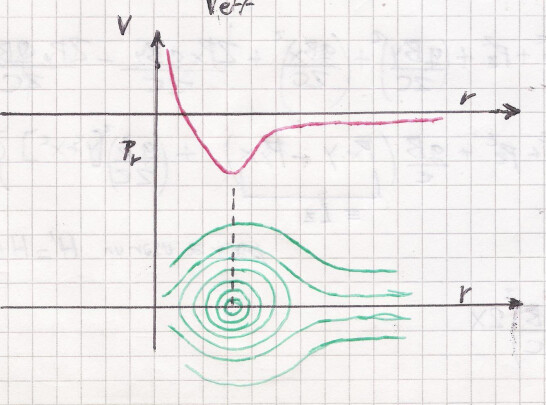
\includegraphics[scale=0.5]{images/fig_mc_problema_1_p96_2.jpg} 
 
\end{ejemplo}


\begin{ejemplo}{\bf Problema 8 P97}
 
\end{ejemplo}









% \bibliographystyle{CBFT-apa-good}	% (uses file "apa-good.bst")
% \bibliography{CBFT.Referencias} % La base de datos bibliográfica

\end{document}
